
%\RequirePackage{pdf15}

\documentclass{beamer}

\usepackage[utf8]{inputenc}

\usepackage{mystyle}

\usepackage{tikz}
\usepackage{pgfplots}
\usepackage{subcaption}

\usepackage{natbib}
\bibliographystyle{apalike}
%\usepackage[style=authortitle,backend=biber]{biblatex}
%\addbibresource{anthology.bib}
%\addbibresource{emnlp2020.bib}
\renewcommand{\footnotesize}{\scriptsize}

\usepackage{tikz-dependency}
\usetikzlibrary{shapes.arrows, positioning, fit, bayesnet,
    arrows,backgrounds,patterns,matrix,calc,shadows,plotmarks,
    shapes,positioning,automata,positioning,spy,scopes,chains,decorations,decorations.pathreplacing}

\newcommand{\FancyUpArrow}{
\begin{tikzpicture}[baseline=-0.3em]
\node[single arrow,draw,rotate=90,single arrow head extend=0.2em,inner
ysep=0.2em,transform shape,line width=0.05em,top color=green,bottom color=green!50!black] (X){};
\end{tikzpicture}}
\newcommand{\FancyDownArrow}{
\begin{tikzpicture}[baseline=-0.3em]
\node[single arrow,draw,rotate=-90,single arrow head extend=0.2em,inner
ysep=0.2em,transform shape,line width=0.05em,top color=red,bottom color=red!50!black] (X){};
\end{tikzpicture}}

\AtBeginSection[]{
  \begin{frame}
  \vfill
  \centering
  \begin{beamercolorbox}[sep=8pt,center,shadow=true,rounded=true]{title}
    \usebeamerfont{title}\insertsectionhead\par%
  \end{beamercolorbox}
  \vfill
  \end{frame}
}

% quotes
\usepackage[style=british]{csquotes}

\def\signed #1{{\leavevmode\unskip\nobreak\hfil\penalty50\hskip1em
  \hbox{}\nobreak\hfill #1%
  \parfillskip=0pt \finalhyphendemerits=0 \endgraf}}

\newsavebox\mybox
\newenvironment{aquote}[1]
  {\savebox\mybox{#1}\begin{quote}\openautoquote\hspace*{-.7ex}}
  {\unskip\closeautoquote\vspace*{1mm}\signed{\usebox\mybox}\end{quote}}

%Information to be included in the title page:
\title{Best-First Rao-Blackwellization}
\author{J Chiu}

\setbeamertemplate{navigation symbols}{} 
\setbeamertemplate{footline}[frame number]

\begin{document}

\begin{frame}[plain]
\titlepage
\end{frame}

\begin{frame}
\frametitle{Gradient Estimation}
\begin{itemize}
\item Goal: optimize
$$\max_\theta \sum_x p_\theta(x)f(x)$$
(optimizing wrt parameters of $f$ is easy)
\item Discrete $x$, expensive evaluation of $f(x)$
    \begin{itemize}
    \item eg $f$ is a giant neural network
    \end{itemize}
\end{itemize}
\end{frame}

\begin{frame}
\frametitle{Gradient Estimators}
\begin{itemize}
\item Score-function estimator (SFE)
    $$\nabla_\theta \sum_x p_\theta(x)f(x)
    = \Es{p_\theta(x)}{f(x)\nabla \log p_\theta(x)}$$
    \begin{itemize}
    \item High variance, consistent
    \item Requires multiple evaluations, better with more compute
    \end{itemize}
\item Continuous relaxation, $x \approx g(\theta, \epsilon)$
    $$\nabla_\theta \sum_x p_\theta(x)f(x)
    \approx \Es{p(\epsilon)}{\nabla_\theta f(g_\theta(\theta, \epsilon))}$$
    \begin{itemize}
    \item Biased, lower variance
    \item Requires low number of evals, less benefit from more compute
    \item Requires relaxable $f$
    \item Stochastic softmax tricks (SST)
    \end{itemize}
\item Focus on improving SFE
    \begin{itemize}
    \item SFE under-explored
    \item Better with more compute is attractive
    \end{itemize}
\end{itemize}
\end{frame}

\begin{frame}
\frametitle{Rao-Blackwellization}
\begin{itemize}
\item Too expensive to enumerate over all $x$ ($f$ is expensive)
\item Reduce effective width of distribution via sub-sampling (red)
\item Enumerate over green portion
\end{itemize}
\centering
\begin{tikzpicture}
\matrix (array) [matrix of nodes,ampersand replacement=\&]
{
p(1) \& p(2) \& p(3) \& p(4)\\
f(1) \& f(2) \& f(3) \& f(4)\\
};
\begin{scope}[on background layer]
\fill[red!10] (array-2-1.north west) rectangle (array-2-2.south east);
\fill[green!10] (array-2-3.north west) rectangle (array-2-4.south east);
\end{scope}
\end{tikzpicture}
\end{frame}


\begin{frame}
\frametitle{Rao-Blackwellization of score function estimator}
\begin{itemize}
\item Condition on values of $f(x)$ for $x\in S$
    \begin{align*}
    &\nabla_\theta \sum_x p_\theta(x)f(x)\\
    &= \Es{p_\theta(x)}{f(x)\nabla \log p_\theta(x)}\\
    &= \sum_{x\in S} p(x)f(x)\nabla \log p_\theta(x)
    + \Es{p_\theta(x \notin S)}{f(x)\nabla \log p_\theta(x)}
    \end{align*}
\item Conditioning on all values $f(x)$ = no variance
\item Want $S$ to have $x$ with high $p(x)f(x)$
    \begin{itemize}
    \item Need to compromise with high $p(x)$
    \item Use heuristic estimate of $f(x)$?
    \item What if $x$ is structured?
    \end{itemize}
\end{itemize}
\end{frame}

\begin{frame}
\frametitle{Structured Setting}
\begin{itemize}
\item In the flat setting, only cared about width
\item In structured setting, can also approximate depth
\end{itemize}
\centering
\begin{tikzpicture}
\matrix (array) [matrix of nodes,ampersand replacement=\&]
{
p(1) \& p(2) \& p(3) \& p(4)\\
f(1) \& f(2) \& f(3) \& f(4)\\
};
\begin{scope}[on background layer]
\fill[red!10] (array-2-1.north west) rectangle (array-2-2.south east);
\fill[green!10] (array-2-3.north west) rectangle (array-2-4.south east);
\end{scope}
\node [above=1cm of array] (flat) {Flat};

\node [right=4cm of flat] (struct) {Structured};
\node[fill=green!10, very thick, circle, minimum size=.7cm] (root) [below=0.5cm of struct] {r};
\node[fill=red!10, very thick, circle, minimum size=.7cm] (0) [below left=0.5cm of root] {0};
\node[fill=green!10, very thick, circle, minimum size=.7cm] (1) [below right=0.5cm of root] {1};
\node[fill=red!10, very thick, circle, minimum size=.7cm] (00) [below left=0.5cm and -.1cm of 0] {00};
\node[fill=red!10, very thick, circle, minimum size=.7cm] (01) [below right=0.5cm and -.1cm of 0] {01};
\node[fill=red!10, very thick, circle, minimum size=.7cm] (10) [below left=0.5cm and -.1cm of 1] {10};
\node[fill=red!10, very thick, circle, minimum size=.7cm] (11) [below right=0.5cm and -.1cm of 1] {11};
\edge[->] {root} {0};
\edge[->] {root} {1};
\edge[->] {0} {00};
\edge[->] {0} {01};
\edge[->] {1} {10};
\edge[->] {1} {11};
\end{tikzpicture}
\end{frame}

\begin{frame}
\frametitle{Best-first Rao-Blackwellization}
\begin{itemize}
\item Modern MCTS
    \begin{itemize}
    \item Prior $p(x)$ (limits width)
    \item Cost-to-go estimate $\tilde{V}(x)$ (limits depth)
    \item Search procedure that links the two
    \end{itemize}
\item Proposal
    \begin{itemize}
    \item In many cases, already have the prior $p(x)$
    \item Estimate cost-to-go with continuous relaxation or cheaper problem-dependent
        weaker model (learned value function approx)
    \item Link the two by marginalization
    \end{itemize}
\end{itemize}
\end{frame}

\begin{frame}
\frametitle{BF RB}
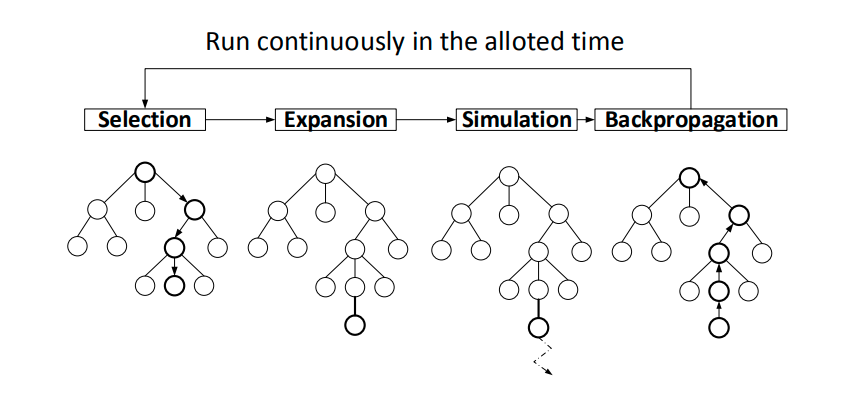
\includegraphics[height=2in]{img/mcts.png}
\end{frame}

\begin{frame}
\frametitle{Minimal Experiment}
Approximate DP when exact is tractable
\begin{itemize}
\item Depth approx: Learn cost-to-go estimate to bound depth in 32k state HMM
    \begin{itemize}
    \item HMM with forward algo that doesnt go all the way to end
    \item Bounded width = prior not important
    \item Experiment with continuous relaxation + learned $\tilde{V}$
        for suffix
    \end{itemize}
\item Width approx: Utilize prior in large-state HMM
    \begin{itemize}
    \item Limit num states considered at each time step
    \end{itemize}
\item Approximations for width + depth
    \begin{itemize}
    \item Probably more useful in PCFGs or other more interesting models
        (massive switching, AR latent)
    \end{itemize}
\end{itemize}
\end{frame}

\begin{frame}
\frametitle{Random thoughts}
\begin{itemize}
\item For exp fam, is this an instance of hypernetworks (ie predicting gradient)?
\end{itemize}
\end{frame}

\begin{frame}[allowframebreaks]
\frametitle{Citations}
%\printbibliography
\bibliography{bib.bib}
\end{frame}

\end{document}
